\chapter{Numerical Solution of Flow Equations}
\label{chapter-three}

\section{Fully-Coupled Point Implicit Method}

The governing equations presented in \erefs{species-cons}{tot-energy-cons} can
be recast in vector form as
%------------------------------------------------------------------------------%
\begin{equation}
	\label{inv_flux_vec}
	\frac{\partial \mathbf{U}}{\partial t}
	+ \nabla\cdot \mathbf{F} = \mathbf{W}
\end{equation}
%------------------------------------------------------------------------------%
 or, in semi-discrete form,
%------------------------------------------------------------------------------%
\begin{equation}
	\label{inv_flux_fv}
	\frac{\partial \mathbf{U}}{\partial t}
	 + \frac{1}{V}\sum\limits_{f}(\mathbf{F}\cdot\mathbf{N})^f = \mathbf{W}
 \end{equation}
%------------------------------------------------------------------------------%
summing over all faces, $f$, in the domain, where V is the cell volume, 
$\mathbf{W}$ is the chemical source term vector, and $\mathbf{N}$ is the face
outward normal vector.  The vectors of conserved variables and fluxes are:
%------------------------------------------------------------------------------%
\begin{equation}
	\begin{matrix}
	\mathbf{U}=\begin{pmatrix}
   		\rho_1\\
		\vdots \\
		\rho_{ns} \\
		\rho u \\
		\rho v \\
		\rho w \\
		\rho E \\
	\end{pmatrix},      &
 	\mathbf{F} = \begin{pmatrix}
		\rho_1  \overline{U} \\
		\vdots \\
		\rho_{ns} \overline{U} \\
		\rho u \overline{U} + p n_x\\
		\rho v \overline{U} + p n_y\\
		\rho w \overline{U} + p n_z\\
		(\rho E + p) \overline{U} \\
	\end{pmatrix}
	\end{matrix}
  \label{fc-variables}
 \end{equation}
%------------------------------------------------------------------------------%
where $\overline{U}$ is the outward pointing normal velocity, $E$ is
the total energy of the mixture per unit mass as defined in
\eref{tot-energy-def}, and $e_s$ is the internal energy of species $s$ as
defined in \eref{int-energy-def}.  By using the Roe FDS scheme,
%------------------------------------------------------------------------------%
\begin{equation}
	\begin{matrix}
		\mathbf{F}^{n+1} \approx \mathbf{F}^n+\frac{\partial \mathbf{F}}{\partial \mathbf{U}}\delta\mathbf{U}^n \\
		\\
		\mathbf{W}^{n+1} \approx \mathbf{W}^n+\frac{\partial \mathbf{W}}{\partial \mathbf{U}}\delta\mathbf{U}^n \\
	\end{matrix}
\end{equation}
%------------------------------------------------------------------------------%
where $\delta\mathbf{U}^n = \mathbf{U}^{n+1}- \mathbf{U}^{n}$.  By using an
implicit time integration, the implicit scheme becomes:
%------------------------------------------------------------------------------%
\begin{equation}
	\frac{\mathbf{\delta U}^n}{\Delta t}+\frac{1}{V}\sum\limits_{f}(\frac{\partial \mathbf{F}^f}{\partial \mathbf{U^L}}\delta\mathbf{U}^L
	+\frac{\partial \mathbf{F}^f}{\partial \mathbf{U^R}}\delta\mathbf{U}^R)^n \mathbf{N}^f
	- \frac{\partial \mathbf{W}}{\partial \mathbf{U}}\delta\mathbf{U}^n
	= -\frac{1}{V}\sum\limits_{f}(\mathbf{F}^f\cdot\mathbf{N}^f)^n + \mathbf{W}^n
\end {equation}
%------------------------------------------------------------------------------%
or, put more simply:
%------------------------------------------------------------------------------%
\begin{equation}
	A\delta\mathbf{U}^n = \mathbf{b}
\end{equation}
%------------------------------------------------------------------------------%
where $A$ is the Jacobian matrix of the fully coupled system, and $\mathbf{b}$
is the residual vector.  For a point implicit relaxation scheme, the Jacobian
matrix can be split into its diagonal and off-diagonal elements, with the latter
moved to the RHS:
%------------------------------------------------------------------------------%
\begin{equation}
\label{decomp_jac}
	A=O+D
\end{equation}
%------------------------------------------------------------------------------%
Each matrix element is a square $(ns+4)\times(ns+4)$ matrix.  One method of
solving this system is a Red-Black Gauss-Seidel scheme\cite{red-black}, where
matrix coefficients with even indices are updated first and, subsequently, the
coefficients with odd indices are updated.  This red-black ordering enables
better vectorization in solving the linear system.  The computational work for
the Gauss-Seidel scheme is dominated by matrix-vector multiplications of
elements of $O$ with $\delta\mathbf{U}$, which are $O(N^2)$ operations, where
$N=ns+4$.  In the next section, it is shown that decoupling the system reduces
these matrix-vector multiplications to $O(M^2 + N)$ operations, where $M=5$ and
$N=ns$.

\section{Decoupled Point Implicit Method}

If the species mass equations are replaced by a single mixture mass equation,
the mixture equations can be separated from the species mass
equations and the conserved variables become
%------------------------------------------------------------------------------%
\begin{equation}
	\begin{matrix}
		\mathbf{U}'=\begin{pmatrix}
			\rho \\
			\rho u \\
			\rho v \\
			\rho w \\
			\rho E
		\end{pmatrix} &
		\mathbf{\hat{U}}=\begin{pmatrix}
			\rho_1 \\
			\vdots \\
			\rho_{ns}
		\end{pmatrix}
	\end{matrix}
  \label{dc-variables}
\end{equation}
%------------------------------------------------------------------------------%
Solving the flux vector is performed in two sequential steps.  The mixture
fluxes are first solved as
%------------------------------------------------------------------------------%
\begin{equation}
  \frac{\partial \mathbf{{U}'}}{\partial t} +
  \frac{1}{V}\sum\limits_{f}(\mathbf{F}'\cdot\mathbf{N})^f = 0
\end{equation}
%------------------------------------------------------------------------------%
followed by the species fluxes as
%------------------------------------------------------------------------------%
\begin{equation}
  \frac{\partial \mathbf{\hat{U}}}{\partial t} +
  \frac{1}{V}\sum\limits_{f}(\mathbf{\hat{F}}\cdot\mathbf{N})^f =
  \mathbf{\hat{W}}
\end{equation}
%------------------------------------------------------------------------------%
Point relaxation uses Red-Black Gauss-Seidel to update the conserved
variables in $\mathbf{U}'$ and all associated auxiliary variables, such as
temperature, pressure, speed of sound, etc.  This is done by holding the
thermo-chemical state constant, and will always result in the relaxation of a
five-equation system.  This does trade an implicit relationship between the mixture
and species equations for an explicit one; thus, this decoupling can have an
impact on the stability of the scheme, especially due to the non-linearity of
the chemical source term\cite{park}.
 
The solution of the species mass equations takes a different form.  Based on the
work of Candler et al.\cite{candler}, the decoupled variables can be rewritten
in terms of mass fraction, as follows:
%------------------------------------------------------------------------------%
\begin{equation}
  \delta \mathbf{\hat{U}}^n =
  \rho^{n+1}\mathbf{\hat{V}}^{n+1}-\rho^n\mathbf{\hat{V}}^n = \rho^{n+1} \delta
  \mathbf{\hat{V}}^n + \mathbf{\hat{V}}^n \delta \rho^n 
\end{equation}
%------------------------------------------------------------------------------%
where $\mathbf{\hat{V}}=(c_1,\hdots,c_{ns})^T$, and $c_s=\rho_s/\rho$ the mass
fraction of species $s$.  While the derivation of the species mass equations is
different for the Roe FDS scheme from that of Steger-Warming proposed by Candler
et al.\cite{candler}, the final result takes a similar form: 
%------------------------------------------------------------------------------%
\begin{gather}
  \hat{F}_{\rho_s} = c_s F'_\rho+(c_s^L-\tilde{c}_s)\rho^L\lambda^+
  + (c_s^R-\tilde{c}_s)\rho^R\lambda^-
  \label{dc_flux}
\end{gather}
%------------------------------------------------------------------------------%
where $F_\rho'$ is the total mass flux computed previously using all
$\mathbf{U}'$ variables, and $\tilde{}$ denotes a Roe-averaged quantity.
Likewise, linearizing the species mass fluxes with respect to the
$\mathbf{\hat{V}}$ variables yields
%------------------------------------------------------------------------------%
\begin{align} 
  \mathbf{\hat{F}}^{n+1} &= \mathbf{\hat{F}}^n +\frac{\partial
  \mathbf{\hat{F}}}{\partial \mathbf{\hat{V}}^L}\delta \mathbf{\hat{V}}^L
  +\frac{\partial \mathbf{\hat{F}}}{\partial \mathbf{\hat{V}}^R}\delta
  \mathbf{\hat{V}}^R \\ \frac{\partial \mathbf{\hat{F}}}{\partial
  \mathbf{\hat{V}}^L} &= \roe F_\rho+(1-w)\rho^L\lambda^+ - \roe \rho^R\lambda^- \\
  \frac{\partial \mathbf{\hat{F}}}{\partial \mathbf{\hat{V}}^R} &=
  ( 1-\roe )F_\rho+(\roe -1)\rho^L\lambda^+ + \roe \rho^R\lambda^-
  \label{d_last}
\end{align}
%------------------------------------------------------------------------------%
A full derivation of \erefs{dc_flux}{d_last}, along with the
definition of $\roe$, is included in Appendix A.  The chemical source term is
linearized in the same manner as the fully coupled scheme; however, the updated
$\mathbf{U}'$ variables are used to evaluate the Jacobian, and the chain rule is
applied to linearize $\mathbf{\hat{W}}$ with respect to the species mass
fractions:
%------------------------------------------------------------------------------%
\begin{equation}
  \mathbf{\hat{W}}^{n+1} = \mathbf{\hat{W}}^n+\frac{\partial
  \mathbf{\hat{W}}}{\partial \mathbf{U}}\bigg|_{\mathbf{U}'} \frac{\partial
  \mathbf{U}}{\partial \mathbf{\hat{V}}} 
\end{equation}
%------------------------------------------------------------------------------%
For simplicity of notation, we define
%------------------------------------------------------------------------------%
\begin{equation}
  C = \frac{\partial \mathbf{\hat{W}}}{\partial
  \mathbf{U}}\bigg|_{\mathbf{U}'} \frac{\partial \mathbf{U}}{\partial
  \mathbf{\hat{V}}}
\end{equation}
%------------------------------------------------------------------------------%
The decoupled system to be solved becomes:
%------------------------------------------------------------------------------%
\begin{gather} 
  \begin{split}
    \rho^{n+1}&\frac{\mathbf{\delta \hat{V}}^n}{\Delta t}
    +\frac{1}{V}\sum\limits_{f}(\frac{\partial \mathbf{\hat{F}}^f}{\partial
    \mathbf{\hat{V}}^L}\delta	\mathbf{\hat{V}}^L
    +\frac{\partial \mathbf{\hat{F}}^f}{\partial \mathbf{\hat{V}}^R}\delta
    \mathbf{\hat{V}}^R)^{n, n+1}\mathbf{N}^f - C^{n, n+1}\delta\mathbf{V}^n \\
    &= -\frac{1}{V}\sum\limits_{f}(\mathbf{\hat{F}}^{n,n+1}\cdot\mathbf{N})^f +
    \mathbf{W}^{n, n+1} -\mathbf{\hat{V}}^n\frac{\delta \rho^n}{\Delta t} -
    R_\rho
  \end{split} \\ 
  R_\rho = -\frac{1}{V}\sum\limits_{f}{\sum\limits_{s}
  {(\hat{F}_{\rho_s}^{n,n+1}\cdot\mathbf{N})}}
\end{gather}
%------------------------------------------------------------------------------%
where $R_\rho$ is included to preserve the constraint that the mass fractions
sum to unity, i.e., $\sum\limits_{s}{c_s}=1$, $\sum\limits_{s}{\delta
c_s}=0$.

\section{Predicted Cost and Memory Savings of the Decoupled Implicit Problem}
\label{sec:predicted-cost-mem-savings}

In decoupling the species equations, the most significant savings comes from the
source term linearization being purely node-based\cite{gnoffo-tp}.  Solving the
mean flow equations is conducted in the same manner as the fully coupled system.
All entries in the Jacobian $A_m$ are linearizations of the mixture equation
fluxes, which results in $5\times5$ matrices. All entries in the Jacobian $A_d$
are linearizations of the species mass fluxes, which results in $ns \times ns$
matrices.  Because there is no interdependence of species, except through the
chemical source term, all contributions due to linearizing the convective flux
are purely diagonal $ns \times ns$ matrices.  Via \eref{decomp_jac}, we
decompose $A_d$ into its diagonal and off-diagonal elements, resulting in the
following linear system:
%------------------------------------------------------------------------------%
\begin{equation}
  \label{dc_sys} 
  \begin{pmatrix} 
    \Box & & & & \\ & \ddots & & & \\ & & \Box \\ & & & \ddots & \\ & & & & \Box
  \end{pmatrix}
  \begin{pmatrix}
    \delta \mathbf{\hat{V}}_1 \\ \vdots \\ \delta \mathbf{\hat{V}}_i \\ 
    \vdots \\ \delta \mathbf{\hat{V}}_{nodes}
  \end{pmatrix}
  =
  \begin{pmatrix}
    \hat{b}_1 \\ \vdots \\ \hat{b}_i \\ \vdots \\ \hat{b}_{nodes} 
  \end{pmatrix}
  -
  \begin{pmatrix}
    (\sum_{j=1}^{N_{nb}}{[\diagdown] \delta\mathbf{\hat{V}}_{j}})_1 \\ \vdots \\
    (\sum_{j=1}^{N_{nb}}{[\diagdown] \delta\mathbf{\hat{V}}_{j}})_i \\ \vdots \\
    (\sum_{j=1}^{N_{nb}}{[\diagdown] \delta\mathbf{\hat{V}}_{j}})_{nodes}
  \end{pmatrix} 
\end{equation} 
%------------------------------------------------------------------------------%
where $\Box$ represents a dense $ns \times ns$ matrix, $[\diagdown]$ represents
a diagonal matrix, and $\delta \mathbf{\hat{V}}_j$  is the decoupled variable
update on the node $j$ that neighbors node $i$, where $N_{nb}$ is the number of
nodes neighboring node $i$.  Thus, the non-zero entries in the off-diagonal
matrix can be reduced from diagonal matrices to vectors.  This results in
significant savings in both computational cost and memory, as the only quadratic
operation left in solving the implicit system is dealing with the diagonal
entries in the Jacobian.  Because the off-diagonal entries significantly
outnumber the diagonal entries, we can expect nearly linear scaling in cost with
the number of species.  If compressed row storage\cite{George} is used to
only store non-zero off-diagonal entries, the relative memory savings in the
limit of a large number of species for the Jacobian is given by
%------------------------------------------------------------------------------%
\begin{equation}
  \label{mem_req_eq}
  \begin{split} 
    Relative\ Memory\ Cost &=
    \frac{size(A_d)}{size(A)} \\ &= \lim_{ns\to\infty}
    \frac{(ns^2+5^2)(N_{nodes})+(ns+5^2)(N_{nz})}{(ns+4)^2(N_{nodes}+N_{nz})} \\
    &= \frac{N_{nodes}}{N_{nodes} + N_{nz}}
  \end{split}
\end{equation}
%------------------------------------------------------------------------------%
where $N_{nodes}$ is the number of nodes, and $N_{nz}$ is the number of non-zero
off-diagonal entries stored using compressed row storage. For a structured grid,
each node has six neighbors in 3D, i.e., $N_{nz} = 6N_{nodes}$; therefore, we can
expect the Jacobian memory required to decrease by a factor of seven using this
decoupled scheme. Interestingly, for a grid that is not purely hexahedra,
$N_{nz} > 6N_{nodes}$; thus, this decoupled scheme provides higher relative
memory savings on unstructured grids than structured grids when using compressed
row storage.

\section{Higher Order Reconstruction}
\label{sec:2nd-order-reconstruction}

To achieve higher-order accuracy, the FUN3D solver uses an extension of the
unstructured MUSCL (U-MUSCL) reconstruction scheme developed by Burg et
al\cite{burg2005higher,burg2003verification}, which is itself an extension of
the Monotonic Upstream-centered Scheme for Conservation Laws (MUSCL) scheme
developed by Van Leer\cite{van1979towards}.  The implementation is a combination
of central differencing and the original U-MUSCL scheme
%------------------------------------------------------------------------------%
\begin{equation}
  \begin{aligned}
    q_L &= q_1 + (1-\kappa)\left[ \phi\left( \pd{q_1}{x}dx + \pd{q_1}{y}dy +
    \pd{q_1}{z}dz \right) \right] + \frac{\kappa}{2}\left( q_2 - q_1 \right) \\
    q_R &= q_2 + (1-\kappa)\left[ \phi\left( \pd{q_2}{x}dx + \pd{q_2}{y}dy +
    \pd{q_2}{z}dz \right) \right] + \frac{\kappa}{2}\left( q_1 - q_2 \right)
  \end{aligned}
  \label{u-muscl}
\end{equation}
%------------------------------------------------------------------------------%
\fref{fig:edge-recons} shows that $q_{L,R}$ are the primitive variables at the
left and right sides of the edge midpoint, where the flux is evaluated,
$q_{1,2}$ are the primitive variables at nodes 1 and 2.
%------------------------------------------------------------------------------%
\begin{figure}[h]
  \centering
  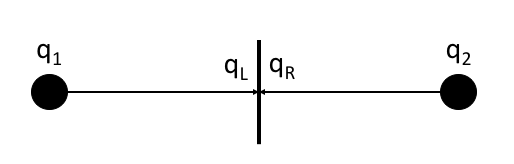
\includegraphics[width=0.5\textwidth]{figures/edge_reconstruction.png}
  \caption{Edge Reconstruction}
  \label{fig:edge-recons}
\end{figure}
%------------------------------------------------------------------------------%
The variable $\phi$ is the result of the scalar flux function, that is required
to preserve monotonicity in the second order reconstruction near
discontinuities.  FUN3D supports a larger variety of flux functions that fall
into two main categories: edge-based limiters, and stencil-based limiters.  The
edge based limiters are evaluated for two nodes at each edge.  Different values
of $\phi$ can exist at each node for edge-based limiter, and the results are not
``freezable'' at each node in FUN3D. Stencil-based limiters are evaluated at
each node, based on the gradients that are computed there.  For these limiters,
the value of $\phi$ is unique to each node and can be stored with the flow
solution as an additional variable.  The frozen state of the limiter is only
re-evaluted if the reconstruction forces a non-physical state at dual volume
interface.

For this study, smooth Van Albada\cite{van1997comparative}, Van
Leer\cite{vatsa2009calibration}, and minmod\cite{roe1986characteristic} flux
limiter functions are used.  Each of these limiters is augmented with a
heuristic pressure limiter by Park\cite{park2008anisotropic}. The choice of
these limiters impacts solution converge and accuracy, and it is important to
note specifics of the smooth Van Albada averaging function is given as
%------------------------------------------------------------------------------%
\begin{equation}
  \phi\left( a, b \right) =
  \frac{(b^2 + \varepsilon^2)a + (a^2 + \varepsilon^2)b}
  {a^2 + b^2 + 2\varepsilon^2}
  \label{van-albada-avg}
\end{equation}
%------------------------------------------------------------------------------%
where $a$ and $b$ are the left and right node gradients, and $\varepsilon$ is
the ``smoothing coefficient''.  This smoothing coefficient is used to tune the
flux limiter to a variety of the problems, and it is advised to be the
reciprocal of the mean aerodynamic chord (MAC) in grid units for
FUN3D\cite{biedron2016fun3d}.  The choice of $\varepsilon$ is critical to some
hypersonic applications involving chemistry, and will be discussed later.

